\chapter{Motivation and Demotivation}\label{s:motivation}

Learners need encouragement to step out into unfamiliar terrain, so this
chapter discusses ways teachers can motivate them. More importantly, it
talks about ways teachers can accidentally \emph{demotivate} them, and how to
avoid doing that.

Our starting point is the difference between \gref{g:extrinsic-motivation}{extrinsic
motivation}, which we feel when we do
something to avoid punishment or earn a reward, and \gref{g:intrinsic-motivation}{intrinsic
motivation}, which is what we feel when we
find something personally rewarding. Both affect most situations---for
example, people teach because they enjoy it and because they get
paid---but we learn best when we are intrinsically motivated
\cite{Wlod2017}. According to \href{https://en.wikipedia.org/wiki/Self-determination\_theory}{self-determination
theory}, the three drivers of intrinsic
motivation are:

\begin{description}
\item[Competence:]
the feeling that you know what you're doing.
\item[Autonomy:]
the feeling of being in control of your own destiny.
\item[Relatedness:]
the feeling of being connected to others.
\end{description}

A well-designed lesson encourages all three. For example, a programming
exercise would give students practice with all the tools they need to
use to solve a larger problem (competence), let them tackle the parts of
that problem in whatever order they want (autonomy), and allow them to
talk to their peers (relatedness).

\begin{aside}{The Problem of Grades}

I've never had an audience in my life. My audience is a rubric.

-- quoted by \href{https://twitter.com/figuralities/status/987330064571387906}{Matt Tierney}

Grades and the way they distort learning are often used as an
example in discussion of extrinsic motivation, but as
\cite{Mill2016a} observes, they aren't going to go away any time
soon, so it's pointless to try to build a system that ignores
them. Instead, \cite{Lang2013} explores how courses that
emphasize grades can incentivize students to cheat, and offers some
tips on how to diminish this effect, while \cite{Covi2017} looks
at the larger problem of balancing intrinsic and extrinsic
motivation in institutional education, and the \href{https://en.wikipedia.org/wiki/Constructive\_alignment}{constructive
alignment} approach advocated in
\cite{Bigg2011} seeks to bring learning activities and learning
outcomes into line with each other.

\end{aside}

\cite{Ambr2010} contains a list of evidence-based methods to motivate
learners. None of them are surprising---it's hard to imagine someone
saying that we \emph{shouldn't} identify and reward what we value---but it's
useful to check lessons against these points to make sure they're doing
at least a few of these things. One strategy I particularly like is to
have students who struggled but succeeded come in and tell their stories
to the rest of the class. Learners are far more likely to believe
stories from people like themselves \cite{Mill2016a}, and people who
have been through your course will always have advice that you would
never have thought of.

\begin{aside}{Not Just for Students}

Discussions of motivation in education often overlook the need to
motivate the \emph{teacher}. Learners respond to a teacher's enthusiasm,
and teachers need to care about a topic in order to keep teaching it,
particularly when they are volunteers. This is another powerful reason
to co-teach (Section~\ref{s:classroom-together}): just as having a
running partner makes it more likely that you'll keep running, having
a teaching partner helps get you up and going on those days when you
have a cold and the projector bulb has burned out and nobody knows
where to find a replacement and why are they doing construction work
today of all days\ldots{}

\end{aside}

Teachers can do other positive things as well. \cite{Bark2014} found
three things that drove retention for all students: meaningful
assignments, faculty interaction with students, and student
collaboration on assignments. Pace and workload (relative to
expectations) were also significant drivers, but primarily for male
students. Things that \emph{didn't} drive retention were interactions with
teaching assistants and interactions with peers in extracurricular
activities. These results may seem obvious, but the reverse would seem
obvious too: if the study had found that extracurricular activities
drove retention, we would also say ``of course''. Noticeably, two of the
four retention drivers (faculty interaction and student collaboration)
take extra effort to replicate online (Chapter~\ref{s:online}).

\section{Authentic Tasks}\label{s:motivation-authentic}

As Dylan Wiliam points out in \cite{Hend2017}, motivation doesn't
always lead to achievement, but achievement almost always leads to
motivation: helping students succeed motivates them far more than
telling them how wonderful they are. We can use this idea in teaching by
creating a grid whose axes are ``mean time to master'' and ``usefulness
once mastered'' (Figure~\ref{f:motivation-what}).

\begin{figure}
\centering
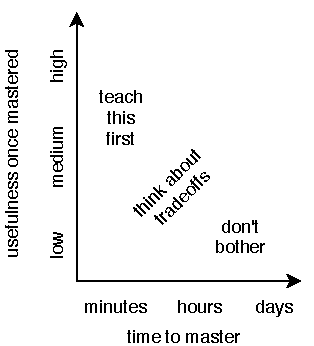
\includegraphics{../../figures/what-to-teach.pdf}
\caption{What to Teach}
\label{f:motivation-what}
\end{figure}

Things that are quick to master and immediately useful should be taught
first, even if they aren't considered fundamental by people who are
already competent practitioners, because a few early wins will build
learners' confidence in their own ability and their teacher's judgment.
Conversely, things that are hard to learn and have little near-term
application should be skipped entirely, while topics along the diagonal
need to be weighed against each other.

Many of the foundational concepts of computer science, such as recursion
and computability, inhabit the ``useful but hard to learn'' corner of this
grid. This doesn't mean that they aren't worth learning, but if our aim
is to convince people that they \emph{can} learn to program, and that doing
so will help them do things that they care about, these big ideas can
and should be deferred. Remember, people often don't want to program for
its own sake: they want to make music or explore changes to family
incomes over time, and (rightly) regard programming as a tax they have
to pay in order to do so.

A well-studied instance of prioritizing what's useful without
sacrificing what's fundamental is the media computation approach
developed at Georgia Tech \cite{Guzd2013}. Instead of printing ``hello
world'' or summing the first ten integers, a student's first program
might open an image, resize it to create a thumbnail, and save the
result. This is an \gref{g:authentic-task}{authentic task}, i.e.,
something that learners believe they would actually do in real life. It
also has a \gref{g:tangible-artifact}{tangible artifact}: if the
image comes out the wrong size, learners have a concrete starting point
for debugging. \cite{Lee2013} describes an adaption of this approach
from Python to MATLAB, while others are building similar courses around
data science, image processing, and biology
\cite{Dahl2018,Meys2018,Ritz2018}.

There will always be tension between giving learners authentic problems
and exercising the individual skills that they will need to solve those
problems. People don't answer multiple choice questions or do Parsons
Problems outside of a classroom, any more than most musicians play
scales over and over again in front of an audience. Finding the balance
is hard, but one easy first step is to make sure that exercises don't
include anything arbitrary or meaningless. For example, programming
examples shouldn't use variables called \texttt{foo} and \texttt{bar}, and if you're
going to have learners sort lines of text, give them album titles or
people's names or something relatable.

\section{Demotivation}\label{s:motivation-demotivation}

\begin{quote}

  Women aren't leaving computing because they don't know what it's like;
  they're leaving because they \emph{do} know. \\
  --- variously attributed

\end{quote}

If you are teaching in a free-range setting, your learners are probably
volunteers, and probably want to be in your classroom. The exercise
therefore isn't how to motivate them, but how to not demotivate them.
Unfortunately, you can do this by accident much more easily than you
might think. For example, \cite{Cher2009} reported four studies
showing that subtle environmental clues have a measurable difference on
the interest that people of different genders have in computing:
changing objects in a CS classroom from those considered stereotypical
of computer science (e.g., Star Trek posters and video games) to objects
not considered stereotypical (e.g., nature poster, phone books) boosted
female undergraduates' interest in CS to the level of their male peers.
Similarly, \cite{Gauc2011} reports a trio of studies showing that
gendered wording commonly employed in job recruitment materials can
maintain gender inequality in traditionally male-dominated occupations.

The three most powerful demotivators for adult learners are
\emph{unpredictability}, \emph{indifference}, and \emph{unfairness}. Unpredictability
demotivates people because if there's no reliable connection between
what they do and what outcome they achieve, there's no reason for them
to try to do anything. Indifference demotivates because learners who
believe that the teacher or educational system doesn't care about them
or the material won't care about it either. And people are also
demotivated if they believe something is unfair, even if it is unfair in
their favor, because they will worry (consciously or unconsciously) that
they will some day find themselves in the group on the losing end
\cite{Wilk2011}. In extreme situations, learners may develop
\gref{g:learned-helplessness}{learned helplessness}: when
repeatedly subjected to negative feedback in a situation that they can't
change, they may learn not to even try to change the things they could.

Here are a few specific things that will demotivate your learners:

\begin{description}
\item[A holier-than-thou or contemptuous attitude]
from a teacher or a fellow learner.
\item[Telling them that their existing skills are rubbish.]
Unix users sneer at Windows, programmers of all kinds make jokes
about Excel, and no matter what web application framework you
already know, some programmer will tell you that it's out of date.
Learners have often invested a lot of time and effort into acquiring
the skills they have; disparaging them is a good way to guarantee
that they won't listen to anything else you have to say.
\item[Diving into complex or detailed technical discussion]
with the most advanced learners in the class.
\item[Pretending that you know more than you do.]
Learners will trust you more if you are frank about the limitations
of your knowledge, and will be more likely to ask questions and seek
help.
\item[Using the J word (``just'') or feigning surprise]
(i.e., saying things like ``I can't believe you don't know X'' or
``you've never heard of Y?''). As discussed in
Chapter~\ref{s:memory}, this signals to the learner that the teacher
thinks their problem is trivial and by extension that they must be
stupid for not being able to figure it out.
\item[Software installation headaches.]
People's first contact with new programming tools, or programming in
general, is often demoralizing, and believing that something is hard
to learn is a self-fulfilling prophecy. It isn't just the time it
takes to get set up, or the feeling that it's unfair to have to
debug something that depends on precisely the knowledge they don't
yet have; the real problem is that every such failure reinforces
their belief that they'd have a better chance of making next
Thursday's deadline if they kept doing things the way they always
have.
\end{description}

It is even easier to demotivate people online than in person, but
there are now evidence-based strategies for dealing with this.
\cite{Ford2016} found that five barriers to contribution on \href{https://stackoverflow.com/}{Stack
Overflow} are seen as significantly more problematic
by women than men: lack of awareness of site features, feeling
unqualified to answer questions, intimidating community size,
discomfort interacting with or relying on strangers, and the
perception that they shouldn't be slacking (i.e., the feeling that
searching for things online wasn't ``real work''). Fear of negative
feedback didn't quite make this list, but would have been the next one
added if the authors weren't quite so strict about their statistical
cutoffs. All of these factors can and should be addressed in both
in-person and online settings using methods like those in
Section~\ref{s:motivation-inclusivity}, and doing so improves outcomes
for everyone \cite{Sved2016}.

\begin{aside}{Productive Failure and Privilege}

Some recent work has explored the notion of productive failure, where
learners are deliberately given problems that can't be solved with the
knowledge they have, and have to go out and acquire new information in
order to make progress \cite{Kapu2016}. Ensuring that learners are
blocked but not frustrated depends more on classroom culture and
expectations than it does on the details of particular exercises.

Productive failure is superficially reminiscent of tech's ``fail fast,
fail often'' mantra, but the latter is more a sign of privilege than of
understanding. People can only afford to celebrate failure if they're
sure they'll get a chance to try again; many of your learners, and
many people from marginalized or underprivileged groups, can't be sure
of that, and talking otherwise is a great way to turn them off.

\end{aside}

\subsection{Impostor Syndrome}\label{s:motivation-impostor-syndrome}

\gref{g:impostor-syndrome}{Impostor syndrome} is the belief that
you aren't really good enough for a job or position---that your
achievements are lucky flukes---and an accompanying fear of someone
finding out. Impostor syndrome is common among high achievers who
undertake publicly visible work, but most people suffer from it
occasionally to some extent. It disproportionately affects members of
under-represented groups: as discussed in Section~\ref{s:pck-now},
\cite{Wilc2018} found that female students with prior exposure to
computing outperformed their male peers in all areas in introductory
programming courses, but were consistently less confident in their
abilities, in part because society keeps signalling in subtle and
not-so-subtle ways that they don't really belong.

Traditional classrooms can fuel impostor syndrome. Schoolwork is
frequently undertaken alone or in small groups, but the results are
shared and criticized publicly; as a result, we rarely see the struggles
of others, only their finished work, which can feed the belief that
everyone else finds it easy. Members of underrepresented groups who
already feel additional pressure to prove themselves may be particularly
affected.

The Ada Initiative has created some \href{https://www.usenix.org/blog/impostor-syndrome-proof-yourself-and-your-community}{guidelines} for
fighting your own impostor syndrome, which include:

\begin{description}
\item[Talk about the issue with people you trust.]
When you hear from others that impostor syndrome is a common
problem, it becomes harder to believe your feelings of being a fraud
are real.
\item[Go to an in-person impostor syndrome session.]
There's nothing like being in a room full of people you respect and
discovering that 90\% of them have impostor syndrome.
\item[Watch your words, because they influence how you think.]
Saying things like, ``I'm not an expert in this, but\ldots{}''
takes away from the knowledge you actually possess.
\item[Teach others about your field.]
You will gain confidence in your own knowledge and skill, and you
will help others avoid some impostor syndrome shoals.
\item[Ask questions.]
Asking questions can be intimidating if you think you should know
the answer, but getting answers eliminates the extended agony of
uncertainty and fear of failure.
\item[Build alliances.]
Reassure and build up your friends, who will reassure and build you
up in return. (And if they don't, find new friends.)
\item[Own your accomplishments.]
Keep actively recording and reviewing what you have done, what you
have built, and what successes you've had.
\end{description}

As a teacher, you can help people with their impostor syndrome by
sharing stories of mistakes that you have made or things you struggled
to learn. This reassures the class that it's OK to find topics hard.
Being open with the group makes it easier to build trust and make
students confident to ask questions. (Live coding is great for this: as
noted in Section~\ref{s:performance-live}, your typos show your class
that you're human.) You can also emphasize that you want questions: you
are not succeeding as a teacher if no one can follow your class, so
you're asking students for their help to help you learn and improve.

\subsection*{Stereotype Threat}

Reminding people of negative stereotypes, even in subtle ways, can make
them anxious about the risk of confirming those stereotypes, which in
turn reduces their performance. This is called
\gref{g:stereotype-threat}{stereotype threat}; \cite{Stee2011}
summarizes what we know about stereotype threat in general and presents
some strategies for mitigating it in the classroom.

Unwelcoming climates demotivate everyone, particularly members of
under-represented groups, but it's less clear that stereotype threat
is the primary cause. Part of the problem is that the term has been
used in many ways \cite{Shap2007}; another is
\href{https://www.psychologytoday.com/blog/rabble-rouser/201512/is-stereotype-threat-overcooked-overstated-and-oversold}{questions} about the replicability of
key studies. What \emph{is} clear is that both instructors and learners
must avoid using language that suggests that some people are natural
programmers and others aren't. Guzdial has called this \href{https://cacm.acm.org/blogs/blog-cacm/189498-top-10-myths-about-teaching-computer-science/fulltext}{the biggest
myth about teaching computer science}, and
\cite{Pati2016} backed this up by showing that people see evidence
for a ``geek gene'' where none exists:

\begin{quote}

Although it has never been rigorously demonstrated, there is a common
belief that CS grades are bimodal. We statistically analyzed 778
distributions of final course grades from a large research university,
and found only 5.8\% of the distributions passed tests of
multimodality. We then devised a psychology experiment to understand
why CS educators believe their grades to be bimodal. We showed 53 CS
professors a series of histograms displaying ambiguous distributions
and asked them to categorize the distributions. A random half of
participants were primed to think about the fact that CS grades are
commonly thought to be bimodal; these participants were more likely to
label ambiguous distributions as ``bimodal''. Participants were also
more likely to label distributions as bimodal if they believed that
some students are innately predisposed to do better at CS. These
results suggest that bimodal grades are instructional folklore in CS,
caused by confirmation bias and instructors' beliefs about their
students.

\end{quote}

Belief that some people get it and some don't is particularly damaging
because of feedback effects. Consciously or unconsciously, teachers tend
to focus their attention on learners who seem to be doing well. That
extra attention increases the odds that they will, while the
corresponding neglect of other learners leaves them further and further
behind \cite{Alvi1999,Brop1983,Juss2005}.

\subsection*{Mindset}

Carol Dweck and others have studied the differences of
\gref{g:fixed-mindset}{fixed mindset} and
\gref{g:growth-mindset}{growth mindset}. If people believe that
competence in some area is intrinsic (i.e., that you either ``have the
gene'' for it or you don't), \emph{everyone} does worse, including the
supposedly advantaged. The reason is that if they don't get it at first,
they figure they just don't have that aptitude, which biases future
performance. On the other hand, if people believe that a skill is
learned and can be improved, they do better on average.

As with stereotype threat, \href{https://educhatter.wordpress.com/2017/03/26/growth-mindset-is-the-theory-flawed-or-has-gm-been-debased-in-the-classroom/}{there are concerns}
that growth mindset has been oversold, or that research is much more
difficult to put into practice than its more enthusiastic advocates
have implied. \cite{Sisk2018} reported two meta-analyses, one
looking at the strength of the relationship between mindset and
academic achievement, the other at the effectiveness of mindset
interventions on academic achievement. The overall effects for both
were weak, but some results supported specific tenets of the theory,
namely, that students with low socioeconomic status or who are
academically at risk might benefit from mindset interventions.

\section{Accessibility}\label{s:motivation-accessibility}

Not providing equal access to lessons and exercises is about as
demotivating as it gets. This is often inadvertent: for example, my
old online programming lessons presented the full script of the
narration beside the slides---but none of the Python source
code. Someone using a \href{https://en.wikipedia.org/wiki/Screen\_reader}{screen reader} would therefore
be able to hear what was being said about the program, but wouldn't
know what the program actually was.

It isn't always possible to accommodate everyone's needs, but it \emph{is}
possible to get a good working structure in place without any specific
knowledge of what specific disabilities people might have. Having at
least some accommodations prepared in advance also makes it clear that
hosts and instructors care enough to have thought about problems in
advance, and that any additional concerns are likely to be addressed.

\begin{aside}{It Helps Everyone}

\href{https://en.wikipedia.org/wiki/Curb\_cut}{Curb cuts} (the small sloped ramps joining a sidewalk to
the street) were originally created to make it easier for the
physically disabled to move around, but proved to be equally helpful
to people with strollers and grocery carts. Similarly, steps taken
to make lessons more accessible to people with various disabilities
also help everyone else. Proper captioning of images, for example,
doesn't just give screen readers something to say: it also makes the
images more findable by exposing their content to search engines.

\end{aside}

The first and most important step in making lessons accessible is to
\emph{involve people with disabilities in decision-making}: the slogan
\emph{\href{https://en.wikipedia.org/wiki/Nothing\_About\_Us\_Without\_Us}{nihil de nobis, sine nobis}} (literally, ``nothing
for us without us'') predates accessibility rights, but is always the
right place to start. A few specific recommendations are:

\begin{description}
\item[Find out what you need to do.]
Each of \href{https://accessibility.blog.gov.uk/2016/09/02/dos-and-donts-on-designing-for-accessibility/}{these posters} offers do's and
don'ts for people on the autistic spectrum, users of screen readers,
and people with low vision, physical or motor disabilities, hearing
exercises, and dyslexia.
\item[Know how well you're doing.]
For example, sites like \href{http://webaim.org/}{WebAIM} allow you to check how
accessible your online materials are to visually impaired users.
\item[Don't do everything at once.]
We don't ask learners in our workshops to adopt all our best
practices or tools in one go, but instead to work things in
gradually at whatever rate they can manage. Similarly, try to build
in accessibility habits when preparing for workshops by adding
something new each time.
\item[Do the easy things first.]
There are plenty of ways to make workshops more accessible that are
both easy and don't create extra cognitive load for anyone: font
choices, general text size, checking in advance that your room is
accessible via an elevator or ramp, etc.
\end{description}

\cite{Coom2012,Burg2015} are good guides to visual design for
accessibility. Their recommendations include:

\begin{description}
\item[Format documents with actual headings and other landmarks,]
rather than just changing font sizes and styles.
\item[Avoid using color alone to convey meaning in text or graphics:]
use color plus cross-hatching or colors that are noticeably
different in grayscale.
\item[Remove all unnecessary elements]
rather than just making them invisible, because screen readers will
still often say them aloud.
\item[Allow self-pacing and repetition]
for people with reading or hearing issues.
\item[Include narration of on-screen action]
in videos.
\end{description}

\subsection{Conduct Revisited}\label{conduct-revisited}

We said in Section~\ref{s:classroom-coc} that classes should
enforce a Code of Conduct like the one in Appendix~\ref{s:conduct}. This
is a form of accessibility: while closed captions make video accessible
to people with hearing disabilities, a Code of Conduct makes lessons
accessible to people who would otherwise be marginalized.

\begin{aside}{Group Signup}

One way to support learners from marginalized groups is to have people
sign up for workshops in groups rather than individually. That way,
everyone in the room will know in advance that they will be with at
least a few people they trust, which increases the chances of them
actually coming. It also helps after the workshop: if people come with
their friends or colleagues, they can work together to use what
they've learned.

\end{aside}

\section{Inclusivity}\label{s:motivation-inclusivity}

\gref{g:inclusivity}{Inclusivity} is a policy of including people
who might otherwise be excluded or marginalized. In computing, it means
making a positive effort to be more welcoming to women,
under-represented racial or ethnic groups, people with various sexual
orientations, the elderly, the physically exercised, the formerly
incarcerated, the economically disadvantaged, and everyone else who
doesn't fit Silicon Valley's white/Asian male demographic.
\cite{Lee2017} is a brief, practical guide to doing that with
references to the research literature. The practices it describes help
learners who belong to one or more marginalized or excluded groups, but
help motivate everyone else as well; while they are phrased in terms of
term-long courses, many can be applied in our workshops:

\begin{description}
\item[Ask learners to email you before the workshop]
to explain how they believe the training could help them achieve
their goals.
\item[Review your notes]
to make sure they are free from gendered pronouns, include
culturally diverse names, etc.
\item[Emphasize that what matters is the rate at which they are learning,]
not the advantages or disadvantages they had when they started.
\item[Encourage pair programming,]
but demonstrate it first so that learners understand the roles
of driver and navigator.
\item[Actively mitigate behavior that some learners may find intimidating,]
e.g., use of jargon or ``questions'' that are actually asked to
display knowledge.
\end{description}

At a higher level, committing to inclusive teaching may mean
fundamentally rethinking content. This is a lot of work, but the rewards
can be significant. For example, \cite{DiSa2014a} found that 65\% of
male African-American participants in a game testing program went on to
study computing, in part because the gaming aspect of the program was
something their peers respected.

Work like this has to be done carefully. \cite{Lach2018} explored two
strategies:

\begin{description}
\item[{\gref{g:community-representation}{Community representation}}]
highlights students' social identities, histories, and community
networks using after-school mentors or role models from students'
neighborhoods, or activities that use community narratives and
histories as a foundation for a computing project.
\item[{\gref{g:computational-integration}{Computational integration}}]
incorporates ideas from the learner's community, e.g., reverse
engineering indigenous graphic designs in a visual programming
environment.
\end{description}

The major risks of these approaches are shallowness (for community
representation), e.g., using computers to build slideshows rather than
do any real computing, and cultural appropriation (for computational
integration), e.g., using practices without acknowledging origins. When
in doubt, ask your learners and members of their community what they
think you ought to do and give them control over content and direction.
We return to this in Chapter~\ref{s:community}.

\subsection{Spoons}\label{spoons}

In 2003, Christine Miserandino started using
\href{https://butyoudontlooksick.com/articles/written-by-christine/the-spoon-theory/}{spoons} as a way to explain what it's like to
live with chronic illness. Healthy people start each day with an
unlimited supply of spoons, but people with lupus or other
debilitating conditions only have a few, and everything they do costs
them one. Getting out of bed? That's a spoon. Making a meal? That's
another spoon, and pretty soon, you've run out.

\begin{quote}

You cannot simply just throw clothes on when you are
sick\ldots{} If my hands hurt that day buttons are out of the
question. If I have bruises that day, I need to wear long sleeves, and
if I have a fever I need a sweater to stay warm and so on. If my hair
is falling out I need to spend more time to look presentable, and then
you need to factor in another 5 minutes for feeling badly that it took
you 2 hours to do all this.

\end{quote}

Spoons are often invisible, but as \href{https://patitsas.blogspot.com/2018/03/spoons-are-form-of-capital.html}{Elizabeth Patitsas has
argued}, people who have a lot can accumulate more,
but people whose supply of spoons is limited may struggle to get ahead
of the game. When you are designing classes and exercises, try to take
into account the fact that some of your learners may have physical or
mental obstacles that aren't obvious. Again, when in doubt, ask your
learners: they almost certainly have more experience with what works
and what doesn't than anyone else.

\subsection{Moving Past the Deficit Model}\label{moving-past-the-deficit-model}

Depending on whose numbers you trust, only 12--18\% of people getting
computer science degrees are women, which is less than half the
percentage seen in the mid-1980s (Figure~\ref{f:motivation-gender}). And
western countries are the odd ones for having such low percentage of
women in computing: women are still often 30--40\% of computer science
students elsewhere \cite{Galp2002,Varm2015}.

\begin{figure}
\centering
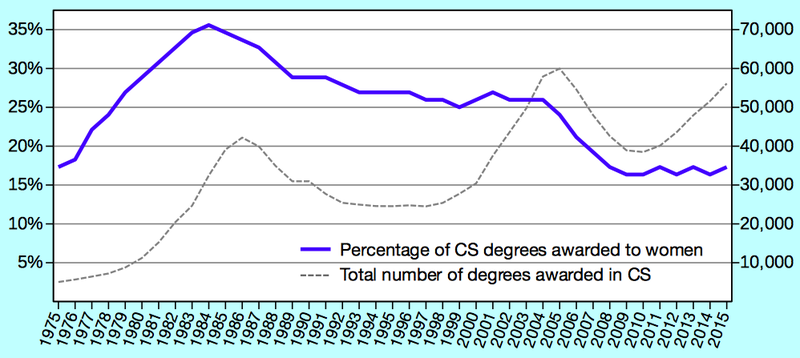
\includegraphics{../../figures/enrollment.png}
\caption{Degrees Awarded and Female Enrollment ({[}Robe2017{]}(\#BIB))}
\label{f:motivation-gender}
\end{figure}

Since it's unlikely that women have changed drastically in the last
thirty years, we have to look for structural causes to understand what's
gone wrong and how to fix it. One reason is the way that home computers
were marketed as ``boys' toys'' starting in the 1980s \cite{Marg2003};
another is the way that computer science departments responded to
explosive growth in enrollment in the 1980s and again in the 2000s by
changing admission requirements \cite{Robe2017}, and as noted at the
start of this section, these factors have excluded many other people as
well. None of these factors may seem dramatic to people who aren't
affected by them, but they act like the steady drip of water on a stone:
over time, they erode motivation, and with it, participation.

The first and most important step toward fixing this is to stop thinking
in terms of a ``leaky pipeline'' \cite{Mill2015}. More generally, we need to
move past a \gref{g:deficit-model}{deficit model} i.e., to stop
thinking that the members of under-represented groups lack something and
are therefore responsible for not getting ahead. Believing that puts the
burden on people who already have to work harder because of the
inequities they face, and (not coincidentally) gives those who benefit
from the current arrangements an excuse not to look at themselves too
closely.

\begin{aside}{Rewriting History}

\cite{Abba2012} describes the careers and accomplishments of the
women who shaped the early history of computing, but have all too
often been written out of that history; \cite{Ensm2003,Ensm2012}
describes how programming was turned from a female into a male
profession in the 1960s, while \cite{Hick2018} looks at how Britain
lost its early dominance in computing by systematically discriminating
against its most qualified workers: women. \cite{Milt2018} is a
good review of all three books. Discussing this can make some men in
computing very uncomfortable; in my opinion, that's a good reason to
do it more often.

\end{aside}

Misogyny in video games, the use of ``cultural fit'' in hiring to excuse
conscious or unconscious bias, a culture of silence around harassment,
and the growing inequality in society that produces preparatory
privilege (Section~\ref{s:classroom-mixed}) may not be any one person's
fault, but they are everyone's responsibility. \href{https://frameshiftconsulting.com/ally-skills-workshop/}{This
workshop} has excellent practical advice on how to be
a good ally in tech; we will return to this topic in
Chapter~\ref{s:community}.

\section{Exercises}\label{s:motivation-exercises}

\subsection*{Authentic Tasks (pairs/15)}

Think about something you did this week that uses one or more of the
skills you teach, (e.g., wrote a function, bulk downloaded data, did
some stats in R, forked a repo) and explain how you would use it (or a
simplified version of it) as an exercise or example in class.

\begin{enumerate}
\item
  Pair up with your neighbor and decide where this exercise fits on a
  2x2 grid of ``short/long time to master'' and ``low/high
  usefulness''.
\item
  Write the task and where it fits on the grid.
\item
  Discuss how these relate back to the ``teach most immediately useful
  first'' approach.
\end{enumerate}

\subsection*{Core Needs (whole class/10)}

Paloma Medina identifies \href{https://www.palomamedina.com/biceps}{six core needs} for people at
work: belonging, improvement (i.e., making progress), choice,
equality, predictability, and significance. After reading her
description of these, order them from most to least significant for
you personally, then compare rankings with your class using 6 points
for most important, 5 for next, and so on down to 1 for least
important. How do you think your rankings compare with those of your
learners?

\subsection*{Implement One Strategy for Inclusivity (individual/5)}

Pick one activity or change in practice from \cite{Lee2017} that you
would like to work on. Put a reminder in your calendar three months in
the future to self-check whether you have done something about it.

\subsection*{Brainstorming Motivational Strategies (think-pair-share/20)}

\begin{enumerate}
\item
  Think back to a programming course (or any other) that you took in
  the past, and identify one thing the instructor did that demotivated
  you, and describe what could have been done afterward to correct the
  situation.
\item
  Pair up with your neighbor and discuss your stories, then add your
  comments to the shared notes.
\item
  Review the comments in the shared notes as a group. Rather than read
  them all out loud, highlight and discuss a few of the things that
  could have been done differently. This will give everyone some
  confidence in how to handle these situations in the future.
\end{enumerate}

\subsection*{Demotivational Experiences (think-pair-share/15)}

Think back to a time when you demotivated a student (or when you were
demotivated as a student). Pair up with your neighbor and discuss what
you could have done differently in the situation, and then share the
story and what could have been done in the group notes.

\subsection*{Walk the Route (whole class/15)}

Find the nearest public transportation drop-off point to your building
and walk from there to your office and then to the nearest washroom,
making notes about things you think would be difficult for someone with
mobility issues. Now borrow a wheelchair and repeat the journey. How
complete was your list of exercises? And did you notice that the first
sentence in this exercise assumed you could actually walk?

\subsection*{Who Decides? (whole class/15)}

In \cite{Litt2004}, Kenneth Wesson wrote, ``If poor inner-city
children consistently outscored children from wealthy suburban homes
on standardized tests, is anyone naive enough to believe that we would
still insist on using these tests as indicators of success?'' Read
\href{https://mobile.nytimes.com/2016/04/10/upshot/why-talented-black-and-hispanic-students-can-go-undiscovered.html}{this article} by Cameron Cottrill, and then
describe an example from your own experience of ``objective''
assessments that reinforced the status quo.

\subsection*{Common Stereotypes (pairs/10)}

You will (still) sometimes hear people say, ``It's so simple that even
your grandmother could use it.'' In pairs, list two or three other
phrases that reinforce stereotypes about computing.

\subsection*{Not Being a Jerk (individual/15)}

\href{https://www.destroyallsoftware.com/blog/2018/a-case-study-in-not-being-a-jerk-in-open-source}{This short article} by Gary Bernhardt rewrites an
unnecessarily hostile message to be less rude. Using it as a model,
find something unpleasant on \href{https://stackoverflow.com/}{Stack Overflow} or some
other public discussion forum and rewrite it to be less repellant.

\subsection*{Saving Face (individual/10)}

Are there any aspects of what you want to teach that members of your
hoped-for audience might be embarrassed to admit to not knowing already?
Are there any that they would rather their peers didn't know they were
learning? If so, what can you do to help them save face?

\subsection*{After the Fact (whole class/15)}

\cite{Cutt2017} surveyed adult computer users about their childhood
activities and found that the strongest correlation between confidence
and computer use were based on reading on one's own and playing with
construction toys with no moving parts (like Lego). Spend a few minutes
searching online for ideas programmers have about how to tell if someone
is going to be a good coder, or what non-coding activities correlate
with programming ability, and see if these two ever come up.

\subsection*{How Accessible Are Your Lessons? (pairs/30)}

In pairs, choose a lesson whose materials are online and independently
rank it according to the do's and don'ts in \href{https://accessibility.blog.gov.uk/2016/09/02/dos-and-donts-on-designing-for-accessibility/}{these
posters}. Where did you and your partner
agree? Where did you disagree? How well did the lesson do for each of
the six categories of user?

\subsection*{Tracing the Cycle (small groups/15)}

\cite{Coco2018} traces a depressingly common pattern in which good
intentions are undermined by an organization's leadership being
unwilling to actually change. Working in groups of 4--6, write brief
emails that you imagine each of the parties involved would send to the
other at each stage in this cycle.
